\section*{Question III}

I used ANOVA model to compare the influence of gender on violence at different levels. Table \ref{t9} shows the model output.

\begin{table}[H]
\centering
\begin{longtable}{lrrrrr}
\toprule
   Source &    DF &    Sum of Squares &    Mean Square &    F Value &    Pr~>~F\\
\endhead
\midrule
   Model &    6 &    2806.376471 &    467.729412 &    Infty &    <.0001\\
   Error &    163 &    0.000000 &    0.000000 &      &     \\
   Corrected Total &    169 &    2806.376471 &      &      &     \\
\bottomrule
\end{longtable}

\begin{longtable}{rrrr}
\toprule
   R-Square &    Coeff Var &    Root MSE &    Score given to incident~Mean\\
\endhead
\midrule
   1.000000 &    0 &    0 &    5.388235\\
\bottomrule
\end{longtable}

\begin{longtable}{lrrrrr}
\toprule
   Source &    DF &    Anova SS &    Mean Square &    F Value &    Pr~>~F\\
\endhead
\midrule
   Sex*Category &    6 &    2806.376471 &    467.729412 &    Infty &    <.0001\\
\bottomrule
\end{longtable}

\caption{ANOVA of the Interaction between Sex of Perpetrator and Category of Incident}
\label{t6}
\end{table}

\begin{table}[H]
\centering
\begin{longtable}{llrrr}
\toprule
   Level of {\newline} Sex of Perpetrator &    Level of {\newline} Category of Incident &    N &    \multicolumn{2}{c}{Score Given to Incident}\\

   ~ &    ~ &    ~ &    Mean &    Std Dev\\
\endhead
\midrule
   F &    1 &    37 &    2.0000000 &    0\\
   F &    2 &    31 &    5.0000000 &    0\\
   F &    3 &    30 &    10.0000000 &    0\\
   M &    1 &    36 &    2.0000000 &    0\\
   M &    2 &    19 &    5.0000000 &    0\\
   M &    3 &    12 &    10.0000000 &    0\\
   M &    4 &    5 &    20.0000000 &    0\\
\bottomrule
\caption{Mean of the Interaction between Sex of Perpetrator and Category of Incident}
\label{t7}

\end{longtable}
\end{table}

\begin{figure}[H]
\centering
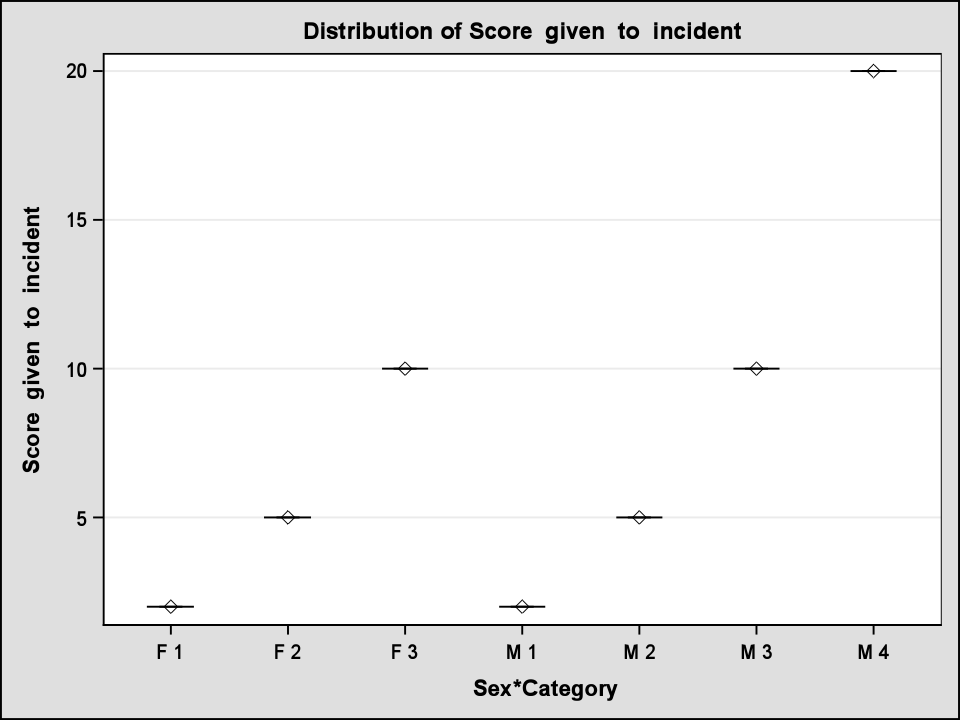
\includegraphics[scale=0.25]{Pic/Q3/3.png}
\caption{ANOVA of the Interaction between Sex of Perpetrator and Category of Incident}
\label{f9}
\end{figure}

According to the table \ref{t6}, we can see p-value is less than 0.0001. Therefore, it is sure that gender has an impact on different levels of violence. The results showed that men were more likely to cause fatal attacks. The option A may be the correct answer.


